%% ------------------------------------------------------------------------- %%
\chapter{Key Concepts}

In this chapter will be presented definitions about the topic, technologies related to it and the principal works in the field of remote attestation. 

\section{Embedded Devices}

One embedded device is a system build to make a specific task. The main difference from normal circuits is the fact that this hardware is programmable, making possible the changes of it functionality only change the program inside it. Normal this devices are low cost, against failures and build work in real time situations. Because they aren't built for general propose, in the most cases they don't have a full operating system running inside it.

Nowadays these devices are changing, they are being connected to the to the internet and making part of the Internet of Things. This makes them vulnerable to attacks and invasions. Make them safe without increasing their cost is one big challenge.

There are embedded system based in processor and microcontrollers.  The microcontrollers (or MCUs from microcontroller unit) are a chip with computational capabilities. In most cases, it is a single integrated circuit (IC) that has inside it the processor, memory, and digital I/O ports. This makes possible the use of same IC in different situations only changing its program. 

This work the focus will be the low-cost embedded system that uses microcontrollers.  Because of its low cost and main objective, this device as limited storage capability and, usually, as a single thread. 

\section{Trust Anchor and Root of Trust}

Trust Anchor and Root of Trust

One of the principal themes related to security is the Trust Anchor. Suppose Alice wants to talk with Bob using an encrypted channel. They can use a symmetric or an asymmetric encryption algorithm to do that. If they choose a symmetric algorithm, they will need to share passphrase before start talking. If they choose an asymmetric algorithm, they need to share their public key in a safe channel. If they share their public keys in an insecure channel, they will not be able to prove the identity of the another. That is, there is a need for a reliable channel before they start the conversation. This channel is the trust anchor.

Another example of a trust anchor can be seen in the TLS (Transport Layer Security) use. In this protocol, there is a need to use previous saved public keys (certificates) before the creation of an encrypted connection. These certificates are usually provided during the operating system (OS) installation. There is a belief that the system during the OS installation this certificates are not corrupted and changed.  This process is the trust anchor of the TLS.

A similar idea of trust anchor can be used in software and hardware verification. When applied to this area it receives the name of Root of Trust. The main idea is to guarantee that the device or software as o knowledge state. Everything that comes after this stade can be predicted and trusted. 

In field software verification are two roots of trust types\cite{minimalistaproacRA}: dynamic and static. In the static one, the verification is made only before the software execution. That is, the software is verified before it is loaded. Suppose a module that verifies if one operation system files have not been modified before boot, this is an example of dynamic roots of trust. A problem related to static method is the fact that it does not give any guarantees about the current state of the software. If any exploits occur after its initialization, it will not be noticed.

The dynamic root of trust is similar to the static one, but it has a way to perform attestation dynamically after the software load. However, it usually uses secret, like a key, to perform the attestation. The software does not have access to this secreted, and there is a need for an authenticated channel to transmit this secret to the device running the software.

\section{Remote Attestation}

Remote attestation is a term used to design the capability to provide attestation cross a network \cite{minimalistaproacRA}. Attestation is the ability to serve clear evidence of something. In the area of security, the evidence is the state of the device. The state is formed by what is present in the device memory in a particular moment.

Remote attestation techniques already have been developed for computers and high-end devices. The Trusted Computing Group (TCG\footnote{https://trustedcomputinggroup.org/}), a computer industry consortium, created a standard, the Trusted Platform Module (TPM\cite{tpm}), to describe architectural elements needed to build a hardware module that provides security capabilities. Among this capabilities is remote attestation.

\begin{figure}[h]
	\centering
	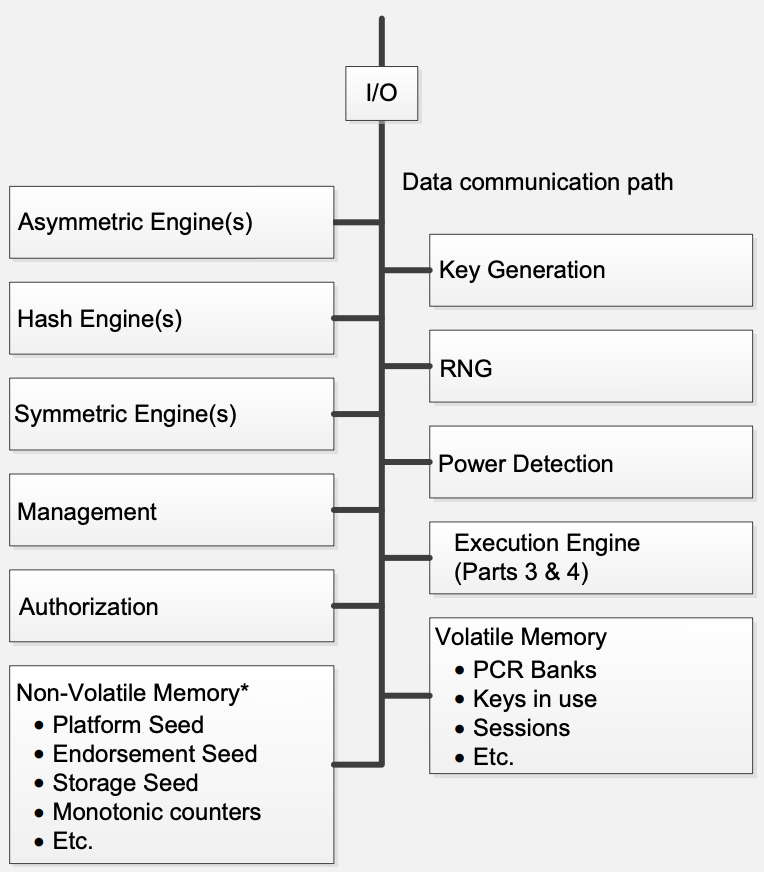
\includegraphics[width=0.45\textwidth]{figuras/tpm}
	\caption{Architectural Overview of TPM. Image from its manual \cite{tpm}.}
	\label{fig:tpm}
\end{figure}

TPM is in its second version. Figure \ref{fig:tpm} shows all components that make part of this module. One use of this module can be to encrypt messages. It has a full encrypt engine inside it and a key stored securely. Commonly, this module is connected with the processor, making possible the exchange of information. 

Within several uses, another interesting is the hardware and software verification. Assume one company do not want modifications in it computers hardware and software. The TMP can make a hash of the bootloader memory and all modules connected with the processor, after that it can sign this information and send to the company. If it suffers any modification, the company will see divergent in the expected data and the receive information. From this, she can stop providing system update or cancel the warranty, for example.

TPM is only one specification of secure cryptoprocessor. Intel and other brand have developed other technics to optimize the secure in its core processors.  However, the cost of this coprocessors is not huge but significant when talking about embed systems.  Usually, microcontrollers that driver the embed system costs a few dollars and the secure cryptoprocessor has practically the same price, making the price almost double. This provides an incentive to study and determine the minimum requirements need to provide a remote attestation. 

The article \cite{minimalistaproacRA} shows the essential elements and function to produce a secure remote attestation protocol. Using the language of this article, in a remote attestation, we have the \textbf{challenger} and the \textbf{prover}. The \textbf{challenger} his the device or computer that verifies the internal state of the \textbf{prover} across the network. The primary objective of the protocol is to allow a not compromised \textbf{prover} to provide an authentication token to the challenger, where it can to find out if the \textbf{prover} is in one expected state.  In case the \textbf{prover} has been modified, the \textbf{challenger} needs to notice that.

To this protocol works there is a need for tree function:
\begin{itemize}
	\item \verb|Setup()|: needs to produce a long key $k$ in a probabilistic way. This function will only be called once. The \textbf{challenger} saves that key and the \textbf{prover} have it, but it can only access it in certain circumstances.
	
	\item \verb|Attest|($k$, $s$): a deterministic algorithm that given one state $s$ of the \textbf{prover} and key $k$, outputs an attestation token $\alpha$. The \textbf{prover} computed this function.
	
	\item \verb|Verify|($k$, $s$, $\alpha$): given a key k, a device state, and an attestation token a. The function returns \verb|True| if \verb|Attest|($k$, $s$) is equal $\alpha$. Otherwise, returns \verb|False|. The \textbf{challenger} computed this function.
\end{itemize}

In a remote attestation verification, the challenger ask for the authentication token to the \textbf{prover}. The \textbf{prover} produces it using \verb|Attest| function, creating the attestation token (in an indirect manner the information of its state). When the \textbf{challenger} receives $\alpha$, it verifies if it can produce the same token, using the \verb|Verify| function.

To this protocol works there is a need to share the key $k$ between the \textbf{challenger} and the \textbf{prover}. We will suppose that this $k$ will be shared in a safe way when the device is manufactory. That is, the key will be write in the device during before it can suffer any attack. The company that produces the device is responsible for generating $k$ and saving it securely. They will use this key after to make the attestation.  

During the protocol is transmitted the attestation token. This transmission occurs over a network and is successive to attacks. If this occurs, the \textbf{prover} will send a token $\alpha$ and the \textbf{challenger} will receives a $\alpha'$. In this case, the \textbf{challenger} will attest the \textbf{prover}  as a violated device (in not know state).  Some technologies, like the Transport Layer Security, can be used to prevent attacks in this connection. One interesting fact to note is that an attacker can save one old authentication token and send this token in a later connection. To prevent this type of attack,  when the \textbf{challenger}  ask for the authentication token, with the request it will send a nonce $n$. This nonce will modify the state of the \textbf{prover} providing a unique state.  This nonce is randomly generated in each authentication token request. The $n$ is not specified in the above function, to make clear the basic idea of the protocol, but in the future, it will be used.

%If the \textbf{prover} suffer one attack, the integrity of the \verb|Attest| function cannot be affected. That is, although the compromised device the \verb|Attest| function needs to work correctly. 

Suppose the \textbf{prover}  suffer an attack, when this happens the state $s$ of the device becomes known by the attacker. With this information he can produce to types of attacks: simulate the \verb|Attest| function a return a correctly $\alpha$; returns a $\alpha$ that is not the real state of the device. To prevent the  attacks mentioned the \verb|Attest| function in the  \textbf{prover} has to have the following properties:

\begin{itemize}
	\item \textbf{Exclusive Access}: only the \verb|Attest| function can have access to key $k$. This makes impossible to forge the token $\alpha$ without running the \verb|Attest|  function. 
	\item \textbf{No Leaks}: after de execution of \verb|Attest| no information of the key $k$ can leak. Otherwise, the key $k$ will become known by the attacker. Cleaning all memory after the function execution can solve this problem.
	\item \textbf{Immutability}: if the \verb|Attest|  can be changed, the attacker can change it to leak the key $k$. 
	\item \textbf{Uninterruptedly}: if during the computation of \verb |Attest| the device suffer one interruption, the key $k$ information can leak.
	\item \textbf{Controlled Invocation}: the  \verb|Attest|  function can only be called by its beginning. Otherwise, the attacker jumps important parts in the \verb|Attest|  code, like the code that disable all interrupts. 
\end{itemize}

The way all these properties will be provided varies according to the device.  Some approaches try to provide all these properties using a software implementation. Unfortunately, the remote attestation using only software has been proved that not work in the internet context.

\section{Works in Remote Attestation for Embedded Devices}

This section has the primary objective to show and discuss the mains works in Remote Attestation for Embedded Devices. It fist subsection will contemplate software remote attestation technics and show why they have been proven to be insecure on the internet. The others subsections focus on some hardware implementations. 

\subsection{Software Remote Attestation}

Several articles tried to construct a remote attestation algorithm using only software, without hardware changes. One of  the main articles in this area is the \textit{Pioneer: Verifying Code Integrity and Enforcing
Untampered Code Execution on Legacy Systems} \cite{pionner}. The basic idea of this article is to send a nonce to the device and for it produces an attestation token based on the device current state. Like in the premises for remote attestation, this token is compared with the expected token to determine if the device is compromised.

However, is not possible to ensure all the guarantee related to the key storage. To work around, the computing time became part of the challenger verification. If the device took too long to calculate the hash, probably the device is attacked. When the Pioneer makes the memory hash, it takes a random look in the memory based in the nonce it receives. If the attacker copies the memory to other place or tried any action to subvert the attestation, this will produce a considerable computation time increase.     The challenger will notice this difference, and it will suspect that the device suffered an attack.

Unfortunately, the connection between the prover and the challenger can vary considerably, making the packet transmission time not be exact and have considerable variance. These technics proposed in Pioneer works well when this connection has a constant transmission time. 

In this implementation, the challenger needs to know accurately the time the device takes to calculate the attestation token. The only way to do this is testing the attestation challenge in a real device. In a real environment with a server verifying a vast number of devices, this process does not become scalable. 

One interesting fact is that the Pioneer solution was made to work on various device types. For example, the article implements the system in an Intel Pentium IV Xeon processor. Pioneer use same ideas previously created in a project called \textit{SWATT: SoftWare-based ATTestation for Embedded Devices}\cite{SWATT}, this is another article that shows a remote attestation technics. The idea in this those implementations is similar, but the main difference is that SWATT works only in embedded devices with simple CPU architectures, like microcontrollers.

Some works have shown failures in the timing based remote attestation systems, like the software one. The \cite{Castelluccia:2009:DSA:1653662.1653711} shows how to forge the SWATT in implementation. Adding simple instructions and reordering the existing ones in the verification source they can forge the authentication token without increasing the computation time significantly. In the conclusion of this article, they declare that software-based attestation is realy challenging to design, but not impossible. The principal reason for this assertion is the fact that small change on the verification code can reduce the verification time and cheat the verifier.

Another article\cite{generic_timming_bug} has tested and simulated attacks to find out the efficiency of the software-based attestation. They showed that depending on the implementation, the attack could be noticed when the prover is not connected directly with the challenger. They also clarified that the majority of generic attacks against timing-based attestation systems are
TOCTOU (time of check to time of use) attacks.  In this class of attacks involving the race condition between checking one condition and using what this condition provides. However, in the end, they conclude that the timing-based remote attestation to be in its infancy.

As seen, the software remote attestations have several problems. It assumes guarantees that are complicated to exist when involving real embed devices on the internet. To make the remote attestation viable was concluded that hardware change is needed. 

\subsection{SMART}

The primary objective of this thesis is to implement and test the hardware and ideas proposed in \textit{SMART: Secure and Minimal Architecture for (Establishing a Dynamic) Root of Trust}\cite{smart}. This article talks about the minimum hardware requirements for embedded devices to make remote attestation viable. 

The basic idea in the article is to change the memory access to get the exclusive access to the key in a ROM memory (read only memory). Changing it, they made the key only accessible when the device program counter points to the first address of the \verb|Attest|. Other changes have also been made to prevent the \verb|Attest| to be executed from its middle. The memory cleaning, to prevent the leak of the key, is implemented as part of the \verb|Attest| function. The uninterruptedly is guaranteed by a software instruction to disable all interruptions at the beginning of the \verb|Attest| function.

The \verb|Attest| function in the device is made using a software SHA-1 hash implementation. It concatenates the device memory and the nonce, send by the challenger and obtain a hash that represents the device state. Also, the function can look only one part of the memory, and this makes possible the attestation of single parts of the device in a relatively short time.

Another functionality that has been added \verb|Attest| function is the capability to the \textbf{challenger} send a function address to be called  at the end of the SMART code execution. This makes possible attest one memory region and, after, call its code in a safety way. The article shows the benefits of this in two examples: the first is to attest the reading of measurements and the second to proof if the device has been successful reset. 

To test the functionality of the idea, they have implemented the smart modifications in two different microcontrollers units: the Atmel AVR and the Texas Instruments MSP430. By the article, adding SMART to both chips caused only a 10\% increase in their respective surface areas. That is, adding the SMART hardware changes do not increase significantly the cost of the device.

All the results from the article are obtained from simulations. The authors did not mention that they have tested the SMART code in FPGAs or ASIC devices. Also, they affirm that more experiments using current implementations need to be performed for better overhead evaluate.

The SMART implementation takes several assumptions. Among them is that the attacker has full control of the device program. It can change it or call other functions. Note that the program can be safely saved in read-only memory, but this not prevent this type of attacks. Some attacks, like a technique called \textit{Return-Oriented Programming} (ROP) \cite{rop}, only change the return pointer in the data memory and reuse the program code in a different memory align to perform the attack. Therefore, in the article are assumed that the attacker has full access and can modify the code outside the protected memory region of SMART.

Another critical assumption as that the device will not suffer any hardware attacks. This is important because if it is possible, the attacker can, for example, make a reset on every time the SMART code is called. Making this successively residual information of the key can leak and than he can obtain the key.

Although carefully designed, some flaws were found in the SMART project \cite{merda}. In SMART, all parameters sent by the challenger can be changed by the attacker.  If this happens, the adversary can make the callable function be inside the smart ROM, making an infinite loop, making a very effective denial-of-service attack without actually controlling the device. This problem is not related in the SMART article but can be simply solved by checking if the end function address is inside de smart ROM before going to it. 

The second flaw is related to the fact that the SMART article is argued that the interruption disable is optional. However, depending on the device's interrupt handler this can cause the leak of the key. Disable the device interrupts during the SMART code execution is a measure to solve this problem.

\subsection{TrustLite}

TrustLite \cite{tlite} is another remote attestation project. It uses SMART as inspiration but has several improvements compared to it. SMART only support one protected area in the ROM memory, in contrast, TrustLite created a Memory Protection Unit (MPU). The MPU is a dedicated hardware table that contains information of several protect memory regions and the address of the that can access it. This hardware unit stays between the CPU core and the address space (including memory and the device peripherals). 

Some advantages of this implementation are the existence of several trust applications. These applications are named \textit{trustlets} by the article. Each \textit{trustlets} are isolated in the sense that no other software on the platform can modify their code. \textit{Trustlets}  data can only be read or modified by other \textit{trustlets} according to the policy described in the (MPU). Also, \textit{trustlets} can validate and the local platform state and other \textit{trustlets}. That is, one \textit{trustlets} can contain the \verb|Attest| to provide the remote attestation features. 

To load the memory access policy to the MPU was developed a \textit{Secure Loader}. This loader works like a \textit{trustlets}, but it is the first to been load and is in a know region of the memory. It is responsible for loading the other  \textit{trustlets}. Another important thing about this loader is the fact that it cleans memory before loading any other code.  This action solves the information leakage on the platform reset,  providing the root of trust. The \textit{Secure Loader} can also be remoted updated. 

In SMART, when on memory violation occurs the hardware make a reset. TrustLite constructs a mechanism to handle memory access violation. On any violation the \textit{trustlets} invalidate the instruction responsible for it. This functionality can prevent an attacker to make the device reset in a critical situation. 

TrustLite can also have insecurity applications. This applications and the \textit{trustlets} can exchange information, creating an interprocess communication. This information exchange can be used, for example, to make one untrusted application (like an input and output control) to be attested. 

The TrustLite was tested in an FPGA. The group that built it used an Intel Siskiyou Peak processor to implement it inside a Xilinx Virtex-6 FPGA. The measure of the hardware extension cost was made based on the number od the FPGA registers and LUTs (more information of LUTs and FPGA can be seen in the section \ref{fpga}), according to the article the cost per module was approximately 8\% in the number of registers and 4\% in the number of LUTs. However, the base core, without any modifications use 552 registers a 14361 LUTs. This total number of LUTS is much higher compared to the 1810 LUTs used in the openMSP430 in the same FPGA. That is, the 622 LUTs used to implement the TrustLite is approximately one-third of the openMSP430 size. This comparison is not exactly, because small changes in the hardware description language or the FPGA syntax settings can produce a significant change in the total number of LUTs. Despite, is still possible to note that TrustLite is more costly than SMART.

In this thesis, it was chosen to be made the SMART implementation because it contains all necessary mechanisms to make the remote attestation viable. Besides that, suppose we want to have multiple applications running in a device. Will be only necessary to attest the code responsible for loading these apps, because if this code is trustworthy every code load by it will also be reliable. Note that will be not possible a dynamic root of trust in this case.

\subsection{SANCUS}

Unlike the two projects mentioned above, SANCUS 2.0 (\textit{A Security Architecture for Low-Cost Networked Embedded Devices})\cite{sancus} project was created to attend a network of devices. The main idea of this project is to provide some capabilities, like software module isolation and remote attestation, in a network of interconnected devices. 

Like the other projects, the SANCUS do not use asymmetric cryptography, because of the high cost of implementing it. However, to provide security the security capabilities, the microprocessor was changed internally to add new special instructions. This kind of changes significantly impacts on the cost of the final device. For example, the remote attestation features were implemented by extending the processor with two more instructions.

Like TrustLite, in SANCUS is possible to load multiple security application inside the device. With application was with own area in memory. Each application was a single key, but this key is no accessible directly, it only can be used by the processor when particular functions are called, like SMART. In SANCUS, every application needs to have a special hardware related to it. This hardware is responsible for saving the application key, the address of de application code and data. Also, it has Memory Access Logic (MAL, as the author), the hardware is used to enforce the memory access rules for a single application and to produce a violation signal if something unexpected happens. 

Differently, from the other projects, the area needed to implement SANCUS is given based on the maximum number of the security application that it can support. The hardware design is evaluated using two different types of logic gates and  three different key sizes. However, in short, we have for SANCUS with only one application, the average increase in hardware size of  90%.

Since the article made changes to the CPU core, it also evaluates the maximum frequency supported by the new microcontroller. The maximum frequency decreases with the number of security applications.  According to the authors, this happens due to the large multiplexer needed to get the module key out of the MAL circuits. Additionally, the maximum frequency decreases much faster when the key size is larger, caused because of the same factor quoted.

All experiments conducted by the authors are made using an XC6SLX25 Spartan-6 FPGA with a speed grade of 2, synthesized using Xilinx ISE Design Suite. This family of FPGAs is the same used in the tests is this thesis. 

\section{FPGA}
\label{fpga}

FPGA is an abbreviation for "field-programmable gate array". This is a special type of integrated circuit created in the 80s, the main difference of others integrates circuits is the possibility to reprogram the circuit using an HDL (hardware description language).

The major benefits are that you can test new hardware and circuits without the need to produce a new integrated circuit. One of the tasks in this work is to change the memory backbone of on microcontroller and test the results. Using the FPGA  the assignment to test the modification became easy because changing it is like reprogram.

There are two principal HDL languages used in the market: Verilog and VHDL. This language is totally differences from normal programming languages.  The principal difference from normal programming languages is the fact that everything is happening in parallel. In this languages, variables are replaced by registers and connected with wires. There are some attempts to convert sequential programming languages, like C, in hardware description languages, like the LegUp High-Level Synthesis project \cite{legup}. But transforming sequential code to hardware normally require big circuit. 

An approach used in used in most FPGA projects is to program a small processor inside it. This processor can be programmed using a sequential programming language. The good thing about this designer is the possibility to connect an hardware in the processor to make specifics tasks. Some companies that produce FPGA's are build processor optimized for their products. One of the most famous projects is MicroBlaze, a 32-bit RISC microprocessor, designed by Xilinx.  A Linux kernel implementation has been made for this processor, making possible to run a Linux inside an FPGA.

Another frequent topic related to FPGAs is the  LookUp Tables (LUTs). Basically, a LUT is a hardware truth table. That is, depending on its input there is a specific logic output. One important FPGA characteristic is it number of LUTs. The LUTs can be classified as the number of accepted inputs. For example, there is 4-inputs LUTs and 6-inputs LUTs. The $k$-input LUT means that it has $k$ configuration pins, making possible a truth table with $2^k$ inputs. 

The capability of saving temporary information is essential for FPGAs. The registers (commonly implemented was flip-flops) are responsible for this property. 

\section{Layers Contemplated}

This work will build a device and program it, involves a different abstraction layers. In figure \ref{fig:layers} is possible to see all the steps and layer in the process of testing and building a microcontroller inside an FPGA.

\begin{figure}[h]
	\centering
	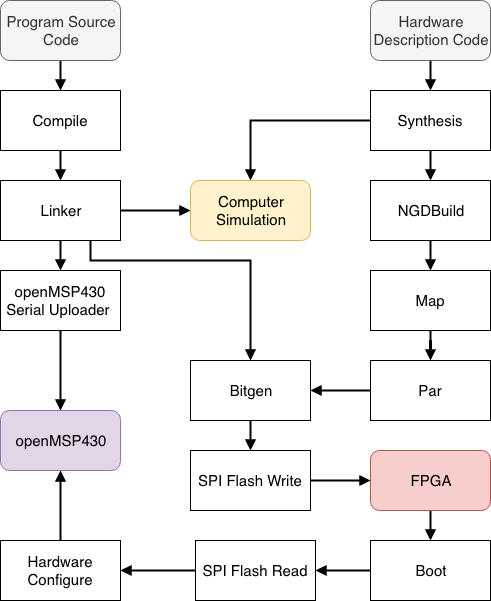
\includegraphics[width=0.6\textwidth]{figuras/layers}
	\caption{Building and loading steps.}
	\label{fig:layers}
\end{figure}


Initially, we have the hardware description language (HDL), responsible for describing all parts of the microcontroller.  In the right part of the image \ref{fig:layers} in a grey box is possible to see the hardware description language. The primary objective is to transform the  HDL source into a file that and be understood and load to the FPGA.

Like a computer program, this language syntax needs to be verified. The synthesis process will check code syntax and analyze the hierarchy of the source design (usually multiple files and modules compose a device).

After the synthesis check, we build a NGC files. That file contains both logical design data and constraints, that is, is the hardware description using only primary elements, like logical port. This file is also known as netlist file.

The Translate process merges all of the input netlists and design constraints and outputs a Xilinx native generic database (NGD) file, which describes the logical design reduced to Xilinx primitives. 

The Map process maps the logic defined by an NGD file into FPGA elements. The output design is a native circuit description (NCD) file that physically represents the design mapped to the components in the FPGA.

The Place and Route (PAR) process takes a mapped NCD file, places and routes the design, and produces an NCD file that is used as input for bitstream generation.

The Bitgen process produces a bitstream for the FPGA device configuration (bin file). This file can be sent to de device flash memory. This update is done via a USB serial cable and is in the diagram as SPI Flash write. After that, when the afpg boot it will read its flash memory, configure it internal gates (Hardware Configuration) and at the end will be a microcontroller. In this thesis case, the openMSP430.

On the left side of the image is the part responsible for managing the source code in C. Initially there is a C code, and we want to transform it into an executable file. For this, there was a need to compile the code, place the assembly generated in specific locations and send it to the device via a serial connection.

One interesting thing is the fact that the executable code can be merged in the FPGA bitstream. In this case, the when the FPGA load the bitstream it will also initialize its memory blocks. 

The last unexplained block is the Computer Simulation. This block is responsible for simulating de hardware and testing its results. This tests usually take a long time, because it sequentially simulates all the hardware parallelism. 

The layer and this diagram can change depending on the tools used in the process. In the image, we have the process specific for the Spartan 6 FPGA family using it manufacture (Xilinx) tools. All FPGA building steps description are based in the Xilinx documentation\footnote{\url{https://www.xilinx.com/support.html\#documentation}}.
